\chapter{IRK: Eguzki-sistema.}

\section{Sarrera.}

Koordenatu kartesiarrak erabiltzearen abantaila.

\section{Kepler-en fluxua.}

\section{Inplementazio berria.}

Eguzki sistemarako honako idei berri bat azalduko dugu. Honako ekuazio diferentziala dugularik,
\begin{equation*}
\dot{y}=k(y)+\epsilon \ g(y)
\end{equation*}

Alde kepleriarraren fluxua ezaguna dugu,
\begin{align*}
\varphi_{\triangle t}^k:&  \ \mathbb{R}^d \ \longrightarrow \mathbb{R}^d  \\
&  y_0 \longrightarrow y_1. 
\end{align*}

Aldagai aldaketa bat egin daiteke,
\begin{align*}
y(t_0+\triangle t) &= \varphi _{\triangle t}^k(z(t_0+\triangle t)), \ \ y(t_0)=z(t_0), \\
z(t_0+\triangle t) &= \varphi _{-\triangle t}^k(y(t_0+\triangle t)).
\end{align*}

Aldagai berriarekiko ekuazio diferentziala mantso aldatzen den funtzioa da,
\begin{align*}
\dot{z}=\epsilon \ r(z,t).
\end{align*} 

Ideia hau bi modutara aplika daiteke,
\begin{enumerate}
\item Gauss inplizituaren integrazio metodoan.
\item Atalen hasieraketa ona lortzeko.
Orokorrean, interpolazio bidezko hasieraketa ona izateko,  urratsa txikia izan behar du (periodo bat baino txikiagoa izan behar du). Teknika hau erabiliz, interpolazioaren errorea $\mathcal{O}(\epsilon)$ mailakoa izango da.

Proposamen honetan hasieraketa $z$ aldagai berria erabiliz era honetan egingo dugu:
\begin{itemize}
\item $Y_{n-1}$ atalei kepler \textbf{denboran atzeratuz}, $Z_{n-1}$ aldagai berriarekiko atalak lortuko ditugu.
\item $Z_{n-1}$ alatak interpolauz, $Z_{n}^{[0]}$ hasieraketak lortuko ditugu.
\item $Z_{n}^{[0]}$ atalei kepler \textbf{denboran aurreratuz}, $Y_{n}^{[0]}$ hasieraketak lortuko ditugu.
\end{itemize}


\end{enumerate}


\begin{figure}[!h]
\centering
\subfloat[Atalen hasieraketa1.]{
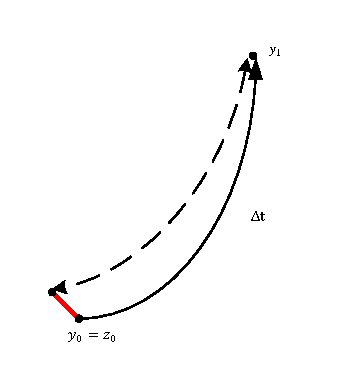
\includegraphics[width=.500\textwidth]{AtalenHasieraketa1}
}
\subfloat[Atalen hasieraketa2.]{
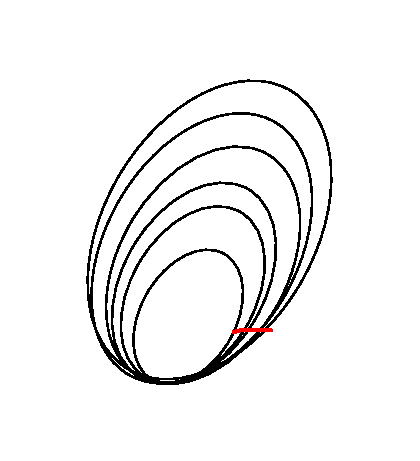
\includegraphics[width=.500\textwidth]{AtalenHasieraketa2}
}
\caption[Atalen hasieraketa.]
        {\small ....        
         \textbf{(a) irudian},                           
         \textbf{(b)} ......        
        }
\label{fig:Atalak12}
\end{figure}   

\begin{figure}[h]
\centerline{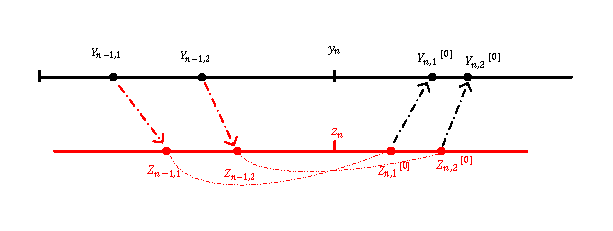
\includegraphics[width=12cm, height=6cm] {AtalenHasieraketa3}}
\caption{Atalen hasieraketa3.}
\label{fig:lau}
\end{figure} 


\section{Zenbakizko esperimentuak.}

\section{Laburpena.}